\begin{figure}[H]
\centering
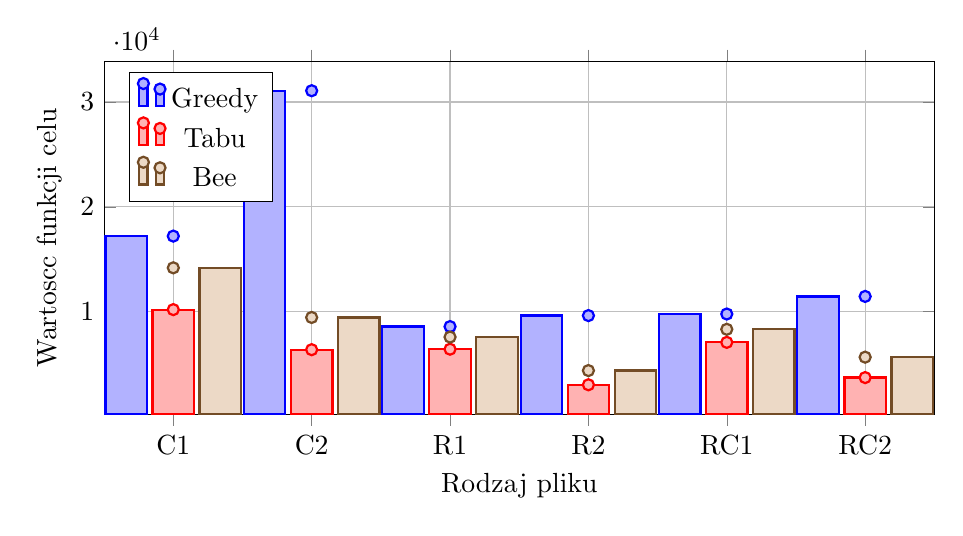
\begin{tikzpicture}
\begin{axis}[
xlabel = {Rodzaj pliku},
ylabel = {Wartoscc funkcji celu},
legend pos = north west,
grid = both,
width=1\linewidth,
height=0.5\linewidth,
ybar,
bar width=15pt,
symbolic x coords={C1,C2,R1,R2,RC1,RC2,},
xtick=data
]
\addplot + [mark = *, thick] coordinates
    {
(C1,17201.11111111111)(C2,31076.875)(R1,8564.25)(R2,9612.272727272728)(RC1,9763.625)(RC2,11443.875)};
\addlegendentry
{Greedy}
\addplot + [mark = *, thick] coordinates
    {
(C1,10183.333333333334)(C2,6357.25)(R1,6405.083333333333)(R2,3008.818181818182)(RC1,7058.25)(RC2,3694.75)};
\addlegendentry
{Tabu}
\addplot + [mark = *, thick] coordinates
    {
(C1,14173.0)(C2,9434.75)(R1,7564.090909090909)(R2,4364.363636363636)(RC1,8304.125)(RC2,5644.875)};
\addlegendentry
{Bee}
\end{axis}
\end{tikzpicture}
\caption
{Porownanie srednich wartosci wynikow algorytmow dla kazdego rodzaju pliku}
\label{fig:mean_comparision}
\end{figure}
